% -*- mode: fundamental -*-

% ****************************************************************

\chapter{RISC-V: Optimizing Drum and Fife}

\markboth{Ch \arabic{chapter}: RISC-V: Optimization}{\copyrightnotice}

\setcounter{page}{1}
% \renewcommand{\thepage}{\arabic{page}}
\renewcommand{\thepage}{\arabic{chapter}-\arabic{page}}

\label{ch_Optimization}

% ****************************************************************

% ----------------
\vspace{2ex}

\centerline{
\includegraphics[width=1in,angle=0]{Figures/Fig_Under_Construction}}

\vspace{2ex}
% ----------------

% ****************************************************************

\section{Introduction}

There are three physical dimensions on which we may want to optimize a
CPU design:

\begin{itemize}

 \item Time (performance): The speed (wall-clock time) at which a
       desired application is executed by the CPU.

 \item Space (area/resources): On ASICs, the silicon area occupied by
       the design.  For ASICS this may be measured in square
       millimeters or in ``number of gates''.  For FPGAs this may be
       measured in LUTs (Lookup Tables), BRAMs, DSPs and so on.
       Smaller is better, for many reasons (better silicon yields,
       lower power consumption, {\etc}.

 \item Energy: the amount of energy consumed to execute a desired
       application. Smaller is better.

\end{itemize}

These are not independent dimensions; improving one dimension often
costs something in another dimension.  Ultimately, a competitive
product specification for a particular target market will define the
acceptable boundaries for each dimension.

We will not say much in this book about energy optimization, even
though it is of course increasingly important in modern times, both in
the macro sense (reduce energy consumption for a greener planet) and
in the micro sense (mobile devices and IoT (Internet of Things)
devices work on battery power or energy harvested from the
environment).  Modern designs have many techniques to slow down or
switch off clocks, and reduce circuit-supply voltage for less critical
or idle circuits, both of which reduce energy consumption.

Regarding Performance, it is important to keep in mind that the
ultimate number that matters is \emph{application performance}, {\ie}
how long does it take to execute an application of interest. One will
often hear other numbers cited as, such as clock speed, instructions
per clock (IPC) or its inverse clocks per instruction (CPI), or total
number of instructions.  All these contribute to application
performance; they do not individually determine application
performance.  Conceptually, the total execution time for an
application is:

\begin{tabbing}
\hmmm \= <exec time> \= $=$ <total number of instrs> \hm \= $\times$ \= $1/$<clock-speed> \hm \= $\times$ \= CPI \\
\\
\hm the units being: \\
\\
      \> seconds     \> $=$ instructions                 \> $\times$ \> seconds/cycle         \> $\times$ \> cycles/instruction
\end{tabbing}

For a given application and a given set of input data, total number of
instructions is a function of the ISA and compiler quality.  ISAs like
x86 or the older DEC PDP-11, DEC Vax, and Motorola 68000 were
\emph{Complex Instruction Sets}, where a single ``CISC'' instruction
could express more work, such as a memory read, an integer op, and a
memory write.  RISC-V is a \emph{Reduced Instruction Set}, where that
same work needs separate ``RISC'' instructions for LOAD, Integer and
STORE.  And, of course, a better compiler may produce a smaller
program (fewer instructions) from the same source code.

CPI is not a constant.  First, it may vary inherently across different
kinds of instructions---an integer ALU instruction may take fewer
cycles than a memory-access instruction or a floating-point
instruction.  Second, even for a particular kind of instruction, CPI
may vary; for example, the number of cycles for a memory-access
instruction may depend on hits/misses in caches, hits/misses in
virtual memory TLBs (Trqnslation Lookaside Buffers), {\etc}.  Third,
an integer that reads a register may stall for a number of cycles
because a preceding instruction has not yet written the register.
Thus, in the above formula, CPI is just an average CPI across the
application.

Clock speed may not be constant; in some implementations, clocks are
slowed down, or even switched off for non-performance-critical
components during intervals that do not demand high performance ({\eg}
``idling'').

The terms in the formula above need simultaneously to be optimized for
the best product.  They are not independent; higher clock speeds
restrict how much ``circuit work'' can be done in a single clock
which, in turn, affects microarchitecture ({\eg} may need to split an
operation into multiple pipeline stages); which, in turn, can affect
instructions/cycle.  A CISC ISA may get more work done with fewer
instructions, but a RISC ISA may be implementable with much higher
clocks speeds and more pipeline parallelism.

Instructions/cycle depends on microarchitecture.  The more parallelism
we can exploit, the higher the instructions/cycles that can be
achieved.  A common term to refer to this measure is ``ILP''
(Instruction-Level Parallelism).

For example, in both Drum and Fife, any particular instruction takes
five or more cycles, from Fetch to Retire.  Drum, having an FSM
microarchitecture, therefore retires one instruction every five or
more cycles.  Fife, which executes many instructions in parallel in
its pipelined microarchitecture, can often retire one instruction per
cycle.

\index{RISC-V!superscalar microarchitecture}
\index{RISC-V!microarchitecture!superscalar}

An advanced microarchitecture with more parallelism is the
\emph{superscalar} microarchitecture, which may fetch and execute 2 or
4 (or more) instructions at a time.

\index{RISC-V!out-of-order microarchitecture}
\index{RISC-V!microarchitecture!out-of-order}

\index{RISC-V!cache!non-blocking}
\index{RISC-V!cache!hit-under-miss}

Another advanced microarchitecture with more parallelism is the
\emph{out-of-order} microarchitecture which may, for example, have
multiple integer execution units, and allow multiple integer
instructions to execute at a time, or even out-of-order depending on
when their input data is available.  The cache in their DMem may
support ``non-blocking caches'' or ``hits-under-misses'' {\ie} for two
memory accesses $a_1$ and $a_2$ that arrive in that order, it permits
$a_2$ to be serviced while $a_1$ may be awaiting a cache-refill due to
a cache-miss.

Superscalarity and Out-of-order microarchitectures are beyond the
scope of this book.  In the rest of this chapter we will discuss
improving the resources and performance of Drum and Fife.

% ****************************************************************

\section{Pipeline traces and visualization to analyze performance}

Before trying to optimize a CPU, we must first analyze and understand
the existing implementation thoroughly so that we can then identify
opportunities for improvement.

\index{RISC-V!Pipeline trace}

The first step is to produce a \emph{pipeline trace}, which has more
fine-grain detail than a mere \emph{instruction trace} (which only
records the trace of instructions retired).  We record, for every
instruction, its transit through \emph{each} step/stage of the FSM
(Drum) or pipeline (Fife).

For example, if we examine the Fife code for \verb|rule rl_Decode| we
see an invocation of a chain of functions:

{\small
\begin{Verbatim}[frame=single, label=src\_Fife/S2\_Decode.bsv]
      log_Decode (rg_flog, y, rsp_IMem);
\end{Verbatim}
}

$\longrightarrow$

{\small
\begin{Verbatim}[frame=single, label=src\_Common/Fn\_Decode.bsv]
   function Action log_Decode (File flog, Decode_to_RR y, Mem_Rsp rsp_IMem);
      ...
      ftrace (flog, y.inum, y.pc, y.instr, "D", $format(""));
      ...
\end{Verbatim}
}

$\longrightarrow$

{\small
\begin{Verbatim}[frame=single, label=src\_Common/Utils.bsv]
function Action ftrace (File         flog, ...)
         ...
	 $fdisplay (flog, "Trace %0d %0d %0h %0h %s", cur_cycle,
		    inum, pc, instr, label, adhoc);
\end{Verbatim}
}

This writes a line like this into the logfile produced by Drum and
Fife when they are simulated:

{\small
\begin{Verbatim}[frame=single, label=log.txt]
...
Trace 6 2 80000008 fe012e23 D
...
\end{Verbatim}
}

which records the fact that on clock tick 6 (cycle 6), the $2^{nd}$
instruction, whose PC is \verb|0x8000_0008|, and whose 32 bits are
\verb|0xfe01_2e23|, was processed in the Decode stage.  Similarly, we
write a trace item for every interesting microarchitectural event for
each instruction.

By studying this code, manually or with analysis software, we can get
an idea of exactly how many cycles each instruction takes, and where
we may be ``losing cycles'', if any.

This trace can also be processed and displayed in a ``pipeline
visualization'' tool.  If we take the pipeline trace \verb|log.txt|
produced by Drum or Fife, we can run it through the Python program
\verb|Log_to_CSV.py| provided with Drum and Fife:

{\small
\begin{Verbatim}[frame=single, label=log.txt]
  $ Tools/Log_to_CSV/Log_to_CSV.py  log.txt  0 100
\end{Verbatim}
}

This selects from instruction 0 through instruction 100 from the
pipeline trace file, and produces a file \verb|log.txt.csv| in the
standard ``comma-separated variables'' data input format that is
accepted by most spreadsheed programs (OpenOffce, Microsoft Excel, Mac
Numbers, Google Sheets).

Figure~\ref{Fig_PipeViz} shows the display, in the Mac Numbers
spreadsheet application, for the pipeline trace of up to the first few
instructions for the ``Hello World!'' C program running on Drum and
Fife, respectively:
\begin{figure}[htbp]
  \centerline{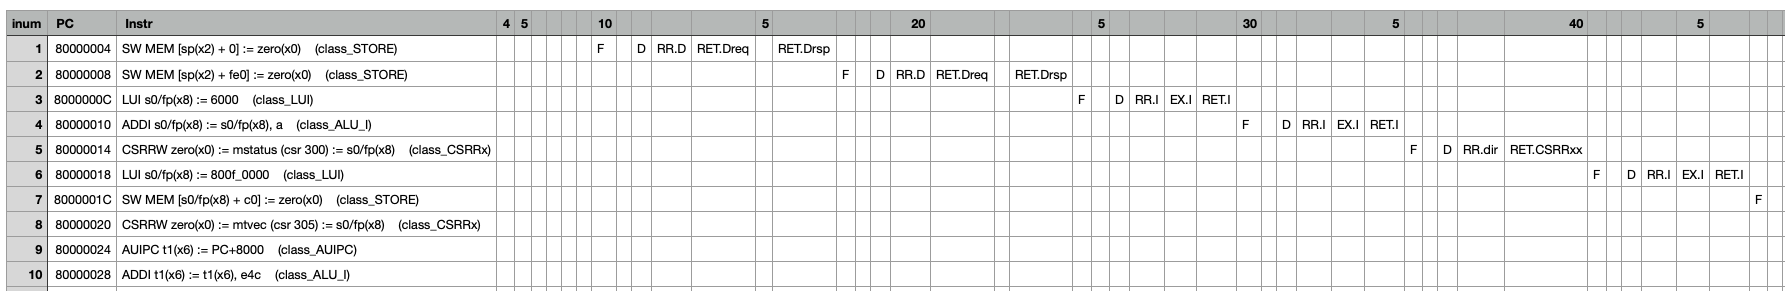
\includegraphics[width=6in,angle=0]{Figures/Fig_PipeViz_Drum}}
  \centerline{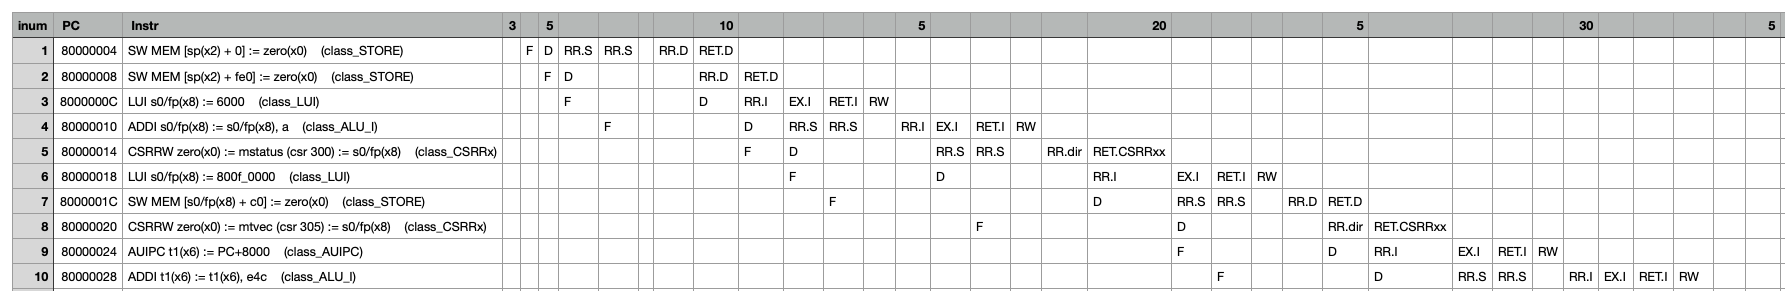
\includegraphics[width=6in,angle=0]{Figures/Fig_PipeViz_Fife}}
  \caption{\label{Fig_PipeViz}
           Visualization of the per-instruction step/stage events in Drum and Fife}
\end{figure}

In both displays, the vertical axis, going downwards, shows
instruction number 1, 2, 3, ...  The horizontal axis, going to the
right, shows the PC and disassembled instruction in the first two
columns, followed by clock ticks.  For each instruction, we see its
instruction numbrer, PC and dissassembly, and then the Drum step/Fife
stage events at the clock tick where the event happened.

We can clearly see the difference between FSM sequenced (Drum) and
pipelined (Fife) behavior.  In Drum, after the first instruction has
completed (``RET.Drsp'' = Retire DMem Response) in tick 6, the Fetch
(``F'') for the second instruction occurs in tick 7.  In Fife, after
the Fetch for the first instruction on tick 4, the Fetch for the
second instruction occurs in tick 5, the very next tick.

Considering IPC, we can see that in Drum, we have barely completed 6
instructions at tick 46, whereas Fife is has finished 10 instruction
by tick 33.  The tradeoff, as suggested earlier, is that Drum takes
far fewer resouces (LUTs, gates) in silicon compared to Fife.

For each instruction, after its Fetch, horizontal gaps indicate lost
cycles, {\eg} an instruction stalling at Register Read because it is
waiting for an earlier instruction to write that register value, or a
memory access waiting for the memory response.  In Fife, we can also
see which instructions were discarded (more lost cycles) due to PC
misprediction or traps.

% ================================================================

\section{Ideas for improving microarchitecture in Drum and Fife}

% ================================================================

\subsection{Wasted clocks due to misprediction}

% ================================================================

\subsection{Wasted clocks due to hazard penalty}

% ================================================================

\subsection{Wasted clocks due to cache misses}

% ================================================================

\subsection{Saving FIFO resources}

Jamming-together mkPipelineFIFOF and mkBypassFIFOF.

% ================================================================

\subsection{Drum: Fusing Decode and RR-Dispatch, fusing some Retire actions}

% ================================================================

\subsection{Fife: Dispatching multiple instructions that write to the same Rd}

\begin{itemize}
 \item Scoreboard bits can can be a small up-down counter, not just Bool
 \item In RR, increment Rd and allow instr to go. Stall if rs1/rs2's counter is not zero.
 \item Current 1-bit is essentially a 1-bit counter.
\end{itemize}

% ================================================================

\subsection{Bypassing: Save a cycle for Redirect in Fetch PC/epoch update}

% ================================================================

\subsection{Bypassing: Save a cycle for in GPRs and Scoreboard for {\tt update\_rd}}

% ================================================================

\subsection{Saving a cycle in Fife by jamming-together Decode and RR-Dispatch}

% ================================================================

\subsection{Saving cycles in Fife Retire by merging exception-handling into other rules}

% ****************************************************************

\section{Exercises}

Many of the above suggestions can be used as exercises by the student,
and actually implemented in Drum and Fife.

% ****************************************************************
